\section{Enzymes}
\subsection{Mode of action of enzymes}
\begin{point}
State that enzymes are globular proteins that catalyse
reactions inside cells (intracellular enzymes) or are secreted to
catalyse reactions outside cells (extracellular enzymes)
\end{point}

\begin{point}
Explain the mode of action of enzymes in terms of an active
site, enzyme–substrate complex, lowering of activation energy
and enzyme specificity, including the lock-and-key hypothesis
and the induced-fit hypothesis
\end{point}
Enzyme molecules have a special feature called an \define{active site}. This is
where the \define{substrate} binds to the enzyme.

The concept where the active site and substrate have very specific 
complementary shapes is called the \define{lock-and-key hypothesis}. The
substrate is held in place by temporary bonds which form between the substrate
and R groups in the active site of the enzyme's amino acids. Due to the 
specificity in this hypothesis, each enzyme only acts on one type of substrate.

New evidence paved way for the \define{induced-fit hypothesis}. This adds the
idea that the enzyme, and sometimes the substrate, can change shape slightly as
the substrate molecules enters the enzyme in order to ensure a perfect fit.

An anzyme may catalyse a reaction where the substrate is split into two 
molecules, or where two substrates are joined into one molecule. The 
substrate(s) bind to the active site, temporarily forming the 
\define{enzyme-substrate complex}, where after the reaction is done, the 
products leave the active site.

An enzyme catalysed reaction reduces the \define{activation energy} of a 
reaction, hence increasing the rate of the reaction.

\begin{point}
Investigate the progress of enzyme-catalysed reactions by
measuring rates of formation of products using catalase and
rates of disappearance of substrate using amylase
\end{point}
Catalase is the enzyme that catalyses the breakdown of hydrogen peroxide into
water and oxygen. We may collect the gaseous product, oxygen to investigate the
rate of this reaction.

A graph is drawn of total volume of oxygen collected against time at which
it is collected.

\begin{center}
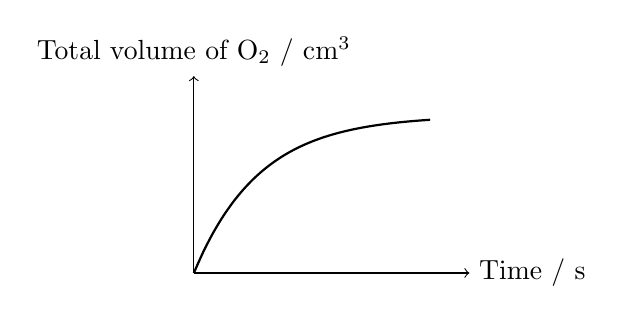
\begin{tikzpicture}[scale=0.5]
  % Axes
  \draw[->] (0,0) -- (7,0) node[right]{Time / s};
  \draw[->] (0,0) -- (0,5) node[above]{Total volume of O$_2$ / cm$^3$};

  % Curve (fast at start, slows down)
  \draw[thick,domain=0:6,smooth,variable=\x] plot ({\x},{4*(1 - exp(-0.6*\x))});
\end{tikzpicture}
\end{center}
Notice that, at the beginning of the reaction the rate of reaction is higher
and it decreases sa the reaction progresses due to decrease in susbtrate
concentration.

We may also do so by measring the rate of disappearance of starch by using
amylase to measure rate of amylase activity.

\begin{point}
Outline the use of a colorimeter for measuring the progress of
enzyme-catalysed reactions that involve colour changes
\end{point}
Colorimeters can give quantitative readings for colors. As it does, we can
investigate colour changes using it.

\subsection{Factors that affect enzyme action}
\begin{point}
	Investigate and explain the effects of the following factors on
	the rate of enzyme-catalysed reactions:
	\begin{itemize}
		\setlength\itemsep{0em}
		\item temperature
		\item pH (using buffer solutions)
		\item enzyme concentration
		\item substrate concentration
		\item inhibitor concentration
	\end{itemize}
\end{point}
\centrebold{Temperature}
\begin{center}
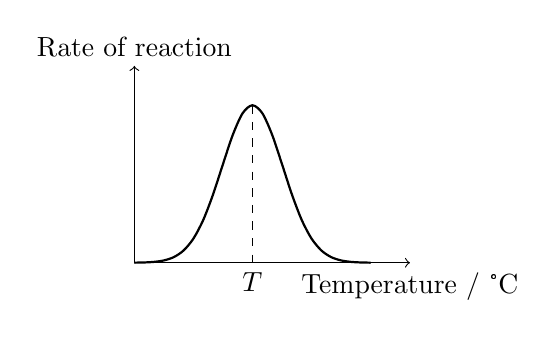
\begin{tikzpicture}[scale=0.5]
	% Axes
	\draw[->] (0,0) -- (7,0) node[below]{Temperature / °C};
	\draw[->] (0,0) -- (0,5) node[above]{Rate of reaction};

	% Curve: rises, peaks, then falls
	\draw[thick,domain=0:6,smooth,variable=\x] 
		plot ({\x},{4*exp(-((\x-3)^2)/1.2)});

	% Label optimum temperature
	\draw[dashed] (3,4) -- (3,0) node[below]{$T$};

\end{tikzpicture}
\end{center}
The above graph shows the trend of all enzyme-catalysed reactions with changes
in temperature.

At low temperatures, the reaction takes place very slowly as the molecules
involved have very little kinetic energies, which means the substrate and 
enzyme collide very infrequently. With greater energy, collisions are more
frequent and more reactions happen. Above a certain temperature however, the
enzyme molecule gains so much kinetic energy that the molecule vibrates to the
extent that some of the bonds holding the molecule in its shape break apart.
It becomes impossible for the enzyme-substrate complex to form as a result.

The temperature at which enzymes have their highest rate of reaction ($T$ in
the given diagram) is called their \define{optimum temperature}.

\centrebold{pH}
\begin{center}
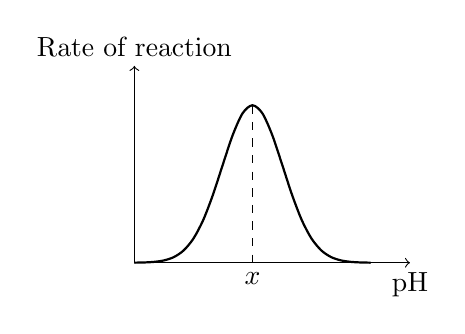
\begin{tikzpicture}[scale=0.5]
	% Axes
	\draw[->] (0,0) -- (7,0) node[below]{pH};
	\draw[->] (0,0) -- (0,5) node[above]{Rate of reaction};

	% Curve: rises, peaks, then falls
	\draw[thick,domain=0:6,smooth,variable=\x] 
		plot ({\x},{4*exp(-((\x-3)^2)/1.2)});

	% Label optimum temperature
	\draw[dashed] (3,4) -- (3,0) node[below]{$x$};

\end{tikzpicture}
\end{center}
pH is a measure of the concentration of hydrogen ions in a solution, where
low pH shows high number of hydrogen ions and vice versa. Ions in amino acids
are affected by the presence of hydrogen and hydroxide ions due to charges,
and as a result pH affects enzyme shapes. As such there is an \define{optimum
pH} at which the enzyme has its highest rate of reaction, where the enzyme's
shape is unscathed.

\centrebold{Enzyme concentration}

Enzyme concentration is directly related to rate of reaction. As enzyme
concentration increases, rate of reaction increases and vice versa.

\centrebold{Substrate concentration}
\begin{center}
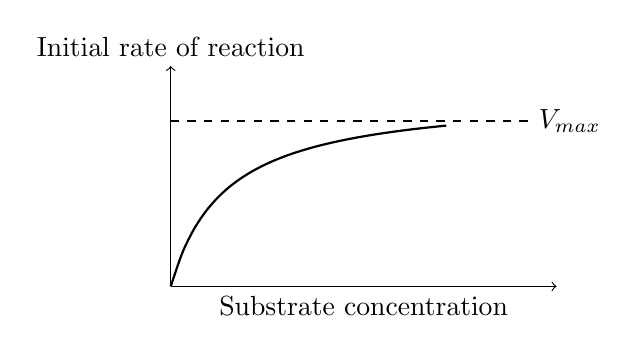
\begin{tikzpicture}[scale=0.7]
  % Axes
  \draw[->] (0,0) -- (7,0) node[midway, below]{Substrate concentration};
  \draw[->] (0,0) -- (0,4) node[above]{Initial rate of reaction};

  % Curve: rapid rise then plateau
  \draw[thick,domain=0:5,smooth,variable=\x]
    plot ({\x},{3.5*(\x)/(1+\x)});

  % Dashed line for Vmax
  \draw[dashed] (0,3) -- (6.5,3) node[right]{$V_{\text{max}}$};

\end{tikzpicture}
\end{center}

If you go on increasing substrate concentration, keeping the enzyme 
concentration constant, there comes a point when every enzyme active site is
full. If more substrate is added, the enzyme simply cannot work faster.

The maximum possible rate is represented as $V_{\text{max}}$, which stands for
maximum velocity.

\centrebold{Inhibitor concentration}

With increase in inhibitor concentration, rate of reaction decreases and vice
versa.

\begin{point}
Explain that the maximum rate of reaction ($V_{\text{max}}$) is used to
derive the Michaelis–Menten constant ($K_m$), which is used to
compare the affinity of different enzymes for their substrates
\end{point}
For $\frac{1}{2}V_{\text{max}}$, the corresponding substrate concentration is
called the Michaelis-Menten constant $K_m$. As such, we can assume that, the
lower the $K_m$, the faster the rate of reaction reaches 
$\frac{1}{2}V_{\text{max}}$ and hence $V_{\text{max}}$. This shows that a lower 
$K_m$ value corresponds to a greater enzyme activity and vice versa.

\begin{point}
Explain the effects of reversible inhibitors, both competitive
and non-competitive, on enzyme activity
\end{point}
Competitive inhibitors have a similar shape to an enzymes substrate and hence
bind to the active site, blocking the substrate itself to bind, slowing down
the rate of the reaction. 

Non-competitive inhibitors do the same, but these
molecules bind to a different part of the enzyme, altering its shape. As a
result, the enzyme cannot carry out its reactions.

\begin{point}
Investigate the difference in activity between an enzyme
immobilised in alginate and the same enzyme free in solution,
and state the advantages of using immobilised enzymes
\end{point}
Enzymes are immobilised when used industrially, in alginate. Substrates are 
made to run \emph{over} these immobilised enzymes, rather than having the
enzymes diffuse freely in a solution.

Immobilised enzymes can be reused, and the products may also be enzyme free.
These enzymes do not denature as easily under pH or temperature changes.
